\tikzset{every picture/.style={line width=0.75pt}} %set default line width to 0.75pt        

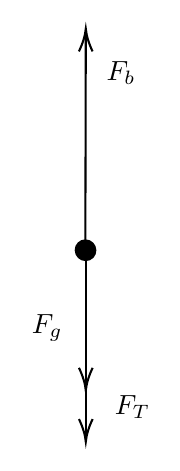
\begin{tikzpicture}[x=0.75pt,y=0.75pt,yscale=-1,xscale=1]
%uncomment if require: \path (0,300); %set diagram left start at 0, and has height of 300

%Shape: Circle [id:dp6675393692095499] 
\draw  [color={rgb, 255:red, 0; green, 0; blue, 0 }  ,draw opacity=1 ][fill={rgb, 255:red, 0; green, 0; blue, 0 }  ,fill opacity=1 ] (317.65,152.72) .. controls (317.6,150.11) and (319.68,148) .. (322.29,148) .. controls (324.9,148) and (327.05,150.11) .. (327.09,152.72) .. controls (327.14,155.33) and (325.06,157.45) .. (322.45,157.45) .. controls (319.84,157.45) and (317.69,155.33) .. (317.65,152.72) -- cycle ;
%Straight Lines [id:da14348149774026253] 
\draw    (322.5,157.45) -- (322.5,243) ;
\draw [shift={(322.5,245)}, rotate = 270] [color={rgb, 255:red, 0; green, 0; blue, 0 }  ][line width=0.75]    (10.93,-3.29) .. controls (6.95,-1.4) and (3.31,-0.3) .. (0,0) .. controls (3.31,0.3) and (6.95,1.4) .. (10.93,3.29)   ;
%Straight Lines [id:da7150129936651202] 
\draw    (322.5,157.45) -- (322.5,218.32) ;
\draw [shift={(322.5,220.32)}, rotate = 270] [color={rgb, 255:red, 0; green, 0; blue, 0 }  ][line width=0.75]    (10.93,-3.29) .. controls (6.95,-1.4) and (3.31,-0.3) .. (0,0) .. controls (3.31,0.3) and (6.95,1.4) .. (10.93,3.29)   ;

%Straight Lines [id:da4333755663247494] 
\draw    (322.29,148) -- (322.5,48) ;
\draw [shift={(322.5,46)}, rotate = 450.12] [color={rgb, 255:red, 0; green, 0; blue, 0 }  ][line width=0.75]    (10.93,-3.29) .. controls (6.95,-1.4) and (3.31,-0.3) .. (0,0) .. controls (3.31,0.3) and (6.95,1.4) .. (10.93,3.29)   ;


% Text Node
\draw (295,182.4) node [anchor=north west][inner sep=0.75pt]    {$F_{g}$};
% Text Node
\draw (335,221.4) node [anchor=north west][inner sep=0.75pt]    {$F_{T}$};
% Text Node
\draw (331,60.4) node [anchor=north west][inner sep=0.75pt]    {$F_{b}$};


\end{tikzpicture}
